\chapter{Суда России и мира}
\label{ch:ships-chapter}

Данная глава посвящена судам, принадлежащих России и другим странам мира. Суда могут иметь различное назначение -- военное или гражданское. Гражданские суда используются во множестве задач: грузоперевозках, рыболовстве, туризме, разведке полезных ископаемых, спасательных работах, а также в спортивных, культурных и других целях. Для хранения такого большого объема информации о судах необходимо вести базы знаний. Одной из таких баз знания является Викиданные. Данная работа направлена на изучение хранимых в Викиданных объектов кораблей и оценке качества и полноты их описания.


\begin{marginfigure}[0.0cm]
  {
    \setlength{\fboxsep}{0pt}%
    \setlength{\fboxrule}{1pt}%
    \fcolorbox{gray}{gray}{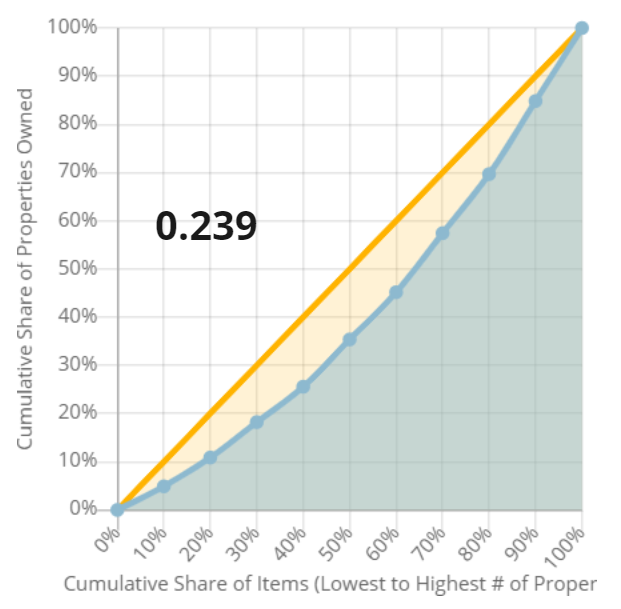
\includegraphics{../graphics/chapter/ship/Russian_ships_topic_imbalance.png}}
  }
  \caption{
    Низкая степень равномерности заполнения по числу свойств объекта Викиданных \href{https://www.wikidata.org/wiki/Q11446}{корабль (Q11446)}.  Данные получены с помощью сервиса ProWD.id, 2020 год. \emph{Коэффициент Джини равен 0.239.}
    }%
    \label{fig:prowd_ships-unbalanced}%
  \end{marginfigure}


\section{Экземпляры объекта ``Корабли''}

Корабль -- это крупное морское судно.

\begin{itemize}
  \item Объект: \href{https://www.wikidata.org/wiki/Q11446}{Корабль (Q11446)}.
  \item Свойство: \href{https://www.wikidata.org/wiki/Property:P31}{Экземпляр (P31)}
\end{itemize}

Построим список всех кораблей на английском и русском языках.

\begin{lstlisting}[ language=SPARQL, label=lst:labeled_langs ]
  #List of ship in Russian
  SELECT ?ship ?shipLabel
  WHERE
  {
    ?ship wdt:P31 wd:Q11446. # instance of ship
    SERVICE wikibase:label { bd:serviceParam wikibase:language "ru". }
  }
\end{lstlisting}

\href{https://query.wikidata.org/#%23List%20of%20ship%20in%20English%20and%20Russian%0ASELECT%20%3Fship%20%3FshipLabel%0AWHERE%0A%7B%0A%20%20%3Fship%20wdt%3AP31%20wd%3AQ11446.%0A%20%20SERVICE%20wikibase%3Alabel%20%7B%20bd%3AserviceParam%20wikibase%3Alanguage%20"ru".%20%7D%0A%7D}{SPARQL-запрос}, 19 820 записей (2017), 50 681 записей (2020).

По данным ProWD больше всего свойств имеет \href{https://www.wikidata.org/wiki/Q281147}{Красин (ледокол, 1916)}.

\begin{lstlisting}[ language=SPARQL, label=lst:labeled_langs ]
  #List of ship from Russia, Soviet Union and Russian Empire
  SELECT ?ship ?shipLabel
  WHERE
  {
    ?ship wdt:P31 wd:Q11446. # instance of ship
                                       # ships belongs to:
    { ?ship wdt:P137/wdt:P17 wd:Q34266 } UNION  # Russian Empire
    { ?ship wdt:P137/wdt:P17 wd:Q15180 } UNION  # Soviet Union
    { ?ship wdt:P137/wdt:P17 wd:Q159 }.         # Russia
    SERVICE wikibase:label { bd:serviceParam wikibase:language "ru". }
  }
\end{lstlisting}

\href{https://query.wikidata.org/#%23List%20of%20ship%20from%20Russia%2C%20Soviet%20Union%20and%20Russian%20Empire%0ASELECT%20%3Fship%20%3FshipLabel%0AWHERE%0A%7B%0A%20%20%3Fship%20wdt%3AP31%20wd%3AQ11446.%20%23%20instance%20of%20ship%0A%20%20%20%20%20%20%20%20%20%20%20%20%20%20%20%20%20%20%20%20%20%20%20%20%20%20%20%20%20%20%20%20%20%20%20%20%20%23%20ships%20belongs%20to%3A%0A%20%20%7B%20%3Fship%20wdt%3AP137%2Fwdt%3AP17%20wd%3AQ34266%20%7D%20UNION%20%20%23%20Russian%20Empire%0A%20%20%7B%20%3Fship%20wdt%3AP137%2Fwdt%3AP17%20wd%3AQ15180%20%7D%20UNION%20%20%23%20Soviet%20Union%0A%20%20%7B%20%3Fship%20wdt%3AP137%2Fwdt%3AP17%20wd%3AQ159%20%7D.%20%20%20%20%20%20%20%20%20%23%20Russia%0A%20%20SERVICE%20wikibase%3Alabel%20%7B%20bd%3AserviceParam%20wikibase%3Alanguage%20"ru".%20%7D%0A%7D}{SPARQL-запрос}, 107 записей (2017), 579 записей (2020).

\section{Плохие и хорошие примеры}

Хорошие примеры объектов кораблей на сайте Викиданных: \href{https://www.wikidata.org/wiki/Q613128}{SMS Moltke}, \href{https://www.wikidata.org/wiki/Q596282}{HMS Hermes}, \href{https://www.wikidata.org/wiki/Q596282}{HMS Barham}.

Плохими примерами объектов кораблей на сайте Викиданных были: \href{https://www.wikidata.org/wiki/Q4264229}{Лихой}, \href{https://www.wikidata.org/wiki/Q18816894}{Николай Вилков}, \href{https://www.wikidata.org/wiki/Q4528362}{Щ-310}.

\section{Полнота Викиданных}

Поиск точного количества кораблей в мире — трудная задача. Ведь данные о некоторых из них являются совершенно секретными, какие-то же — это частные судна и информации о них тоже нет. Предположим, что общее число кораблей равно 1 210 895, как указано в базе данных судов\footnote{База данных судов, 2017}. \href{https://query.wikidata.org/#%23List%20of%20ships%20in%20English%20and%20Russian%0ASELECT%20%3Fship%20%3FshipLabel%0AWHERE%0A%7B%0A%20%20%3Fship%20wdt%3AP31%20wd%3AQ11446.%0A%20%20SERVICE%20wikibase%3Alabel%20%7B%20bd%3AserviceParam%20wikibase%3Alanguage%20"en".%20%7D%0A%7D}{SPARQL-запрос} показал только 19 886 записей, что составляет только 1,6\% от общего числа кораблей..

Что касается российских кораблей, то актуальный боевой корабельный состав ВМФ России\footnote{Актуальный список корабельного состава ВМФ России на 16 октября 2017 г., 2017} выдает 72 подводные лодки, а также 211 боевых кораблей и катеров. В то время, когда \href{https://query.wikidata.org/#%23List%20of%20ships%20%0ASELECT%20%3Fship%20%3FshipLabel%0AWHERE%0A%7B%0A%20%20%3Fship%20wdt%3AP31%20wd%3AQ11446.%0A%20%20SERVICE%20wikibase%3Alabel%20%7B%20bd%3AserviceParam%20wikibase%3Alanguage%20"en".%20%7D%0A%20%20%20%20%20%20%20%20%20%20%20%20%20%20%20%20%20%20%20%20%20%20%20%20%20%20%20%20%20%20%20%20%20%20%20%20%20%23%20ships%20are%3A%0A%20%20%7B%20%3Fship%20wdt%3AP17%20wd%3AQ34266%20%7D%20UNION%20%20%23%20Russian%20Empire%0A%20%20%7B%20%3Fship%20wdt%3AP17%20wd%3AQ15180%20%7D%20UNION%20%20%23%20Soviet%20Union%0A%20%20%7B%20%3Fship%20wdt%3AP17%20wd%3AQ159%20%7D.%20%20%20%20%20%20%20%20%20%23%20Russia%0A%7D%0A}{запрос} выдало всего 25 записей.

И в первом, и во втором случае разница между фактическим количеством кораблей и результатом запросов огромная, что говорит о неполноте Викиданных.


\section{Заполнение свойств военных кораблей}

Требуется найти и заполнить сто объектов кораблей, связанных с Россией и участвовавших в каких-либо военных конфликтах.


\begin{lstlisting}[ language=SPARQL, label=lst:labeled_langs ]
  #List of ships with countries and war conflicts in Russian
  SELECT ?ship ?shipLabel ?countryLabel ?conflict ?conflictLabel
  WHERE
  {
    ?ship wdt:P31 wd:Q11446;        # instance of ship
          wdt:P137/wdt:P17 ?country;         # belongs to country
          wdt:P607 ?conflict.       # engaged in some conflict
    SERVICE wikibase:label { bd:serviceParam wikibase:language "ru". }
  }
\end{lstlisting}

\href{https://query.wikidata.org/#%23List%20of%20ship%20with%20countries%20and%20war%20conflicts%20in%20Russian%0ASELECT%20%3Fship%20%3FshipLabel%20%3FcountryLabel%20%3Fconflict%20%3FconflictLabel%0AWHERE%0A%7B%0A%20%20%3Fship%20wdt%3AP31%20wd%3AQ11446%3B%0A%20%20%20%20%20%20%20%20wdt%3AP17%20%3Fcountry%3B%20%20%20%20%20%20%20%20%20%23%20belongs%20to%20country%0A%20%20%20%20%20%20%20%20wdt%3AP607%20%3Fconflict.%20%20%20%20%20%20%20%23%20engaged%20in%20some%20conflict%0A%20%20SERVICE%20wikibase%3Alabel%20%7B%20bd%3AserviceParam%20wikibase%3Alanguage%20"ru".%20%7D%0A%7D}{SPARQL-запрос}, 1300 записей на 28 октября 2017 года, 23:12; 16 записей (2020).

\href{https://query.wikidata.org/#%23List%20of%20ships%20with%20countries%20and%20war%20conflicts%20in%20Russian%0ASELECT%20%3Fship%20%3FshipLabel%20%3FcountryLabel%20%3Fconflict%20%3FconflictLabel%0AWHERE%0A%7B%0A%20%20%3Fship%20wdt%3AP31%20wd%3AQ11446%3B%20%20%20%20%20%20%20%20%23%20instance%20of%20ship%0A%20%20%20%20%20%20%20%20wdt%3AP137%2Fwdt%3AP17%20%3Fcountry%3B%20%20%20%20%20%20%20%20%20%23%20belongs%20to%20country%0A%20%20%20%20%20%20%20%20wdt%3AP607%20%3Fconflict.%20%20%20%20%20%20%20%23%20engaged%20in%20some%20conflict%0A%20%20SERVICE%20wikibase%3Alabel%20%7B%20bd%3AserviceParam%20wikibase%3Alanguage%20"ru".%20%7D%0A%7D}{SPARQL-запрос}, 1400 записей на 29 октября 2017 года, 23:39; 3586 записей (2020).

При заполнении свойств военных кораблей, а именно военных конфликтов, в которых они участвовали, указывалось свойство \href{https://www.wikidata.org/wiki/Property:P607}{conflict (P607)} (война/сражение). В то же время военные конфликты и военные операции, которые являются частью войн, являются разными понятиями. Заполненные данных о кораблях можно условно по делить на два типа:

\begin{enumerate}
  \item Объекты, у которых военные операции объединены с военными конфликтами. Например, у \href{https://www.wikidata.org/wiki/Q4148613}{эсминца Гремящий} девять войн/сражений. Такое большое число связано с тем, что корабль принял участие во многих \href{https://ru.wikipedia.org/wiki/Арктические_конвои}{арктических конвоях}, которые являются военными операциями.
  \item Объекты, у которых военные операции отделены от военных конфликтов. Например, у британского крейсера \href{https://ru.wikipedia.org/wiki/HMS_Trinidad_(1940)}{HMS Trinidad} участие в военной кампании и арктическом конвое указаны как часть Второй мировой войны с помощью квалификатора \href{https://www.wikidata.org/wiki/Property:P1012}{including (P1012)}. Таким образом, в Викиданных у этого крейсера указана одна война/сражение.
\end{enumerate}

Для первого типа заполнения в скриптах с поиском у кораблей свойства \ref{https://www.wikidata.org/wiki/Property:P607}{conflict (P607)} будет отображаться больше войн/сражений, чем при втором. Но в этом случае операция \href{https://ru.wikipedia.org/wiki/Одесская_оборона_(1941)}{Одесская оборона} будет стоять наряду с \href{https://ru.wikipedia.org/wiki/Великая_Отечественная_война}{Великой Отечественной войной}, хотя она является частью этой войны. В такой ситуации выводимые данные будут не точными.

Для второго типа заполнения в скриптах можно четко различить войну и военную операцию, также выводимые на графике данные будут точнее.


\begin{lstlisting}[ language=SPARQL, label=lst:labeled_langs ]
  #List of ship with countries and war conflicts in Russian
  SELECT ?ship ?shipLabel ?countryLabel ?conflict ?conflictLabel
  WHERE
  {
    ?ship wdt:P31 wd:Q11446;        # instance of ship
          wdt:P137/wdt:P17 ?country;        # belongs to operator
          wdt:P607 ?conflict.       # engaged in some conflict
    
    { ?country wdt:P17 wd:Q34266 } UNION  # Russian Empire
    { ?country wdt:P17 wd:Q15180 } UNION  # Soviet Union
    { ?country wdt:P17 wd:Q159 }.         # Russia
    
    SERVICE wikibase:label { bd:serviceParam wikibase:language "ru". }
  }
\end{lstlisting}

\href{https://query.wikidata.org/#%23List%20of%20ship%20with%20countries%20and%20war%20conflicts%20in%20Russian%0ASELECT%20%3Fship%20%3FshipLabel%20%3FcountryLabel%20%3Fconflict%20%3FconflictLabel%0AWHERE%0A%7B%0A%20%20%3Fship%20wdt%3AP31%20wd%3AQ11446%3B%20%20%20%20%20%20%20%20%23%20instance%20of%20ship%0A%20%20%20%20%20%20%20%20wdt%3AP137%2Fwdt%3AP17%20%3Fcountry%3B%20%20%20%20%20%20%20%20%23%20belongs%20to%20operator%0A%20%20%20%20%20%20%20%20wdt%3AP607%20%3Fconflict.%20%20%20%20%20%20%20%23%20engaged%20in%20some%20conflict%0A%20%20%0A%20%20%7B%20%3Fcountry%20wdt%3AP17%20wd%3AQ34266%20%7D%20UNION%20%20%23%20Russian%20Empire%0A%20%20%7B%20%3Fcountry%20wdt%3AP17%20wd%3AQ15180%20%7D%20UNION%20%20%23%20Soviet%20Union%0A%20%20%7B%20%3Fcountry%20wdt%3AP17%20wd%3AQ159%20%7D.%20%20%20%20%20%20%20%20%20%23%20Russia%0A%20%20%0A%20%20SERVICE%20wikibase%3Alabel%20%7B%20bd%3AserviceParam%20wikibase%3Alanguage%20"ru".%20%7D%0A%7D}{Выполнить запрос (ru)} - было 105 результатов, 07:38, 6 ноября 2017; 86 записей (2020).